\documentclass[14pt, a4paper]{article}
\usepackage{extsizes} % Enables ability to change font size
\usepackage{indentfirst}

% Font settings
\usepackage[utf8]{inputenc}
\usepackage[T1,T2A]{fontenc}
\usepackage[russian,english]{babel}
\usepackage{tempora}
\linespread{1.5}

% Indentation settings
\usepackage[a4paper, left=30mm, right=15mm, top=20mm, bottom=20mm]{geometry}

% Paragraph offset size
\setlength\parindent{1.25cm}

% Configure links
\usepackage[spaces,hyphens]{url}
\usepackage[colorlinks,allcolors=black]{hyperref}
\urlstyle{same}

% Configure colors
\usepackage{color}
\definecolor{lightgray}{rgb}{0.9647058823529412,0.9725490196078431,0.9803921568627451}
\definecolor{gray}{rgb}{0.48627450980392156,0.48627450980392156,0.48627450980392156}
\definecolor{blue}{rgb}{0.0,0.3607843137254902,0.7843137254901961}
\definecolor{green}{rgb}{0.27058823529411763,0.49411764705882355,0.2901960784313726}
\definecolor{purple}{rgb}{0.65, 0.12, 0.82}

% Configure listings
\usepackage{listings}
\lstset{
  basicstyle=\fontsize{12}{13}\ttfamily,
  columns=fullflexible,
  breaklines=true,
  postbreak=\mbox{\textcolor{red}{$\hookrightarrow$}\space},
  escapeinside={\%*}{*)},
  backgroundcolor=\color{lightgray},
  numberstyle=\footnotesize,
  tabsize=2,
  xleftmargin=4ex
}

% Use style=linesWithNumbers to enable lines enumerating
\lstdefinestyle{linesWithNumbers}{
  numbers=left,
  numberstyle=\color{gray}
}

\lstdefinelanguage{JavaScript}{
  keywords={break, continue, delete, else, for, function, if, in, let,
  new, return, this, typeof, var, void, while, with, const, false, null, true, boolean, number, undefined,
  Array, Boolean, Date, Math, Number, String, Object},
  keywordstyle=\color{blue}\bfseries,
  commentstyle=\color{green}\ttfamily,
  stringstyle=\color{purple}\ttfamily,
  sensitive,
  morecomment=[s]{/*}{*/},
  morecomment=[l]//,
  morecomment=[s]{/**}{*/}, % JavaDoc style comments
  morestring=[b]',
  morestring=[b]"
  fontadjust=true,
  numbersep=10pt,
}[keywords, comments, strings]

\usepackage{caption}

\def\code#1{\texttt{#1}} % Inline code

\usepackage{graphicx}

\begin{document}
\selectlanguage{russian}

\tableofcontents
\pagebreak

\addcontentsline{toc}{section}{Введение}
\section*{Введение}
Babel $-$ это JavaScript-транскомпилятор, используемый в основном для преобразования кода ECMAScript 
2015+ (ES6+) в более раннюю версию JavaScript. Инструмент применяется для того, чтобы иметь 
возможность использовать все современные возможности языка при разработке и одновременно с этим 
обеспечить совместимость написанного кода со старыми версиями браузеров, не поддерживающими эти новые 
возможности.

Особенностью Babel является его модульная архитектура $-$ трансформации, применяемые к коду, 
описываются в отдельных плагинах, которые можно подключать по отдельности, либо в виде пресета 
(группы плагинов). Также существует возможность создавать свои собственные плагины, чем я и собираюсь
 заняться в рамках выпускной квалификационной работы.

Целью этой работы является создание плагина, позволяющего использовать собственные синтаксические 
конструкции в контексте JavaScript кода. Моя мотивация к выбору этой тематики заключается в желании 
получить более глубокое представление о транспиляции программного кода, а также об устройстве работы 
наиболее популярного из JavaScript транспайлеров $-$ Babel. Кроме того, проделанная работа может 
послужить доказательством концепции (proof of concept), если возникнет желание предложить внесение 
вышеупомянутых собственных синтаксических конструкций в стандарт языка JavaScript.

Данная работа состоит из двух частей. В первой части представлен обзор

\pagebreak
\section{Базовые концепции}
\subsection{ECMAScript и JavaScript}
ECMAScript $-$ это скриптовый язык программирования общего назначения, стандартизированный международной 
организацией ECMA в спецификации ECMA-262 \cite{ecma-262}. Спецификация ECMA-262 содержит правила и рекомендации, 
которые должны соблюдаться языком программирования, чтобы он считался совместимым с ECMAScript.

ES $-$ сокращение от ECMAScript. Каждая версия языка ECMAScript именуется с помощью сокращения ES и 
номера версии соответственно. Первая версия языка (ES1)  была выпущена в 1997 году. Самое значимое 
обновление язык получил с выходом стандарта версии ES6 (он же ES2015), в котором был добавлен новый 
синтаксис для описания классов, а также поддержка стрелочных функций, констант,  переменных с ограниченной областью 
видимости и так далее.

JavaScript $-$ язык программирования, являющийся реализацией стандарта ECMA-262. Другими словами, 
JavaScript расширяет язык ECMAScript, привнося в него дополнительные возможности.

\subsection{Babel}
Согласно официальной документации \cite{documentation} Babel является JavaScript компилятором. Однако, 
использование термина компилятор здесь не совсем уместно. Обычно под компилятором понимается программа, 
преобразующая исходные тексты программ, написанные на языке программирования высокого уровня, 
непосредственно в машинные инструкции. В большинстве других источников Babel называют транспайлером. 
Транспайлер (или транскомпайлер) $-$ это программа, преобразующая исходный код на одном языке высокого 
уровня в код на другом языке высокого уровня. В случае с Babel $-$ производятся преобразования между 
различными версиями языка JavaScript.

Необходимость в транспилировании JavaScript заключается в желании обеспечить совместимость написанного 
кода с максимальным числом браузеров. Дело в том, что большинство браузеров используют свой отдельный 
JavaScript интерпретатор (в Chrome используется V8, в Firefox $-$ SpiderMonkey, а в Internet Explorer $-$ Chakra), 
и каждый из этих интерпретаторов поддерживает свое независимое подмножество возможностей ES6 (2015). Это 
означает, что код одного и того же приложения может работать для пользователей одних браузеров и не 
работать для пользователей других. Именно эту проблему решает транспиляция кода с помощью Babel. Она 
позволяет использовать современный стандарт JavaScript при разработке и одновременно с этим обеспечить 
широкую поддержку браузеров.

Помимо решения проблемы совместимости, транспайлеры играют важную роль в процессе принятия решений 
комитетом TC39, группой специалистов, ответственных за разработку стандарта ECMAScript. Например, 
Babel поддерживает все экспериментальные возможности языка (находящиеся на рассмотрении комитетом), 
для того чтобы собрать отзывы от реальных пользователей, которые в свою очередь могут повлиять на 
решение членов комитета.


\subsection{Аналоги Babel}
Среди аналогов Babel можно выделить 2 наиболее масштабных, на мой взгляд, проекта: 
\textit{Traceur} и \textit{JSTransform}.

\textit{Traceur} \cite{traceur} - JavaScript транспайлер, предшественник Babel, презентованный компанией Google в 2011 году. 
Ввиду того, что проект перестал поддерживаться разработчиками с 2016 года, Traceur имеет заметно 
меньшую поддержку новых возможностей JavaScript по сравнению с Babel. Также на ограниченную 
функциональность повлиял архитектурный подход, выбранный разработчиками Traceur. Все проводимые над 
кодом трансформации заданы жестко внутри самого транспайлера, что несколько усложняет процесс расширения 
функциональности инструмента. В отличие от монолитной архитектура Traceur, Babel использует систему 
плагинов, с помощью которых описываются трансформации кода. Плагины могут разрабатываться отдельно 
от самого транспайлера и подключаться по востребованию.

\textit{JSTransform} \cite{jstransform} $-$ утилита, разрабатываемая в компании Facebook с 2013 по 2015 год, и изначально используемая 
в процессе сборки проектов на ReactJS. В первую очередь JSTransform позиционировался как
инструмент именно для создания и последующего применения к исходному коду собственных синтаксических преобразований, 
нежели как готовый ES6-to-ES5 транспайлер. По этой причине проект по умолчанию включал лишь небольшой 
набор предопределенных трансформаций. C 2015 проект JSTransform не поддерживается разработчиками и 
не рекомендуется к использованию.

*Вывод по аналогам*

\subsection{Принцип работы Babel}

Транспилирование исходного кода с помощью Babel происходит в три последовательных этапа: парсинг текста 
исходного кода, трансформация и генерация результирующего кода. Прежде чем подробнее рассмотреть каждый из 
этих этапов, необходимо ознакомиться с таким понятием, как \textit{абстрактное синтаксическое дерево}, 
так как оно используется на каждом из трех этапов транспиляции.

\subsubsection*{Абстрактное синтаксическое дерево}

Абстрактное синтаксическое дерево (abstract syntax tree, AST) $-$ это древовидное представление структуры исходного кода, написанного
на каком либо языке программирования. Внутренние узлы такого дерева представляют операторы языка 
программирования, а листья $-$ соответствующие им операнды.  

Дерево называется абстрактным потому, что оно, в отличие от дерева разбора, содержит лишь упрощенную модель программы. При построении
AST игнорируются элементы, не влияющие на семантику исходного кода. Например, в абстрактном синтаксическом
дереве будут отсутствовать группирующие скобки, так как группировка операндов и так явно задана с помощью структуры дерева.

\begin{figure}[h!]
  \centering
  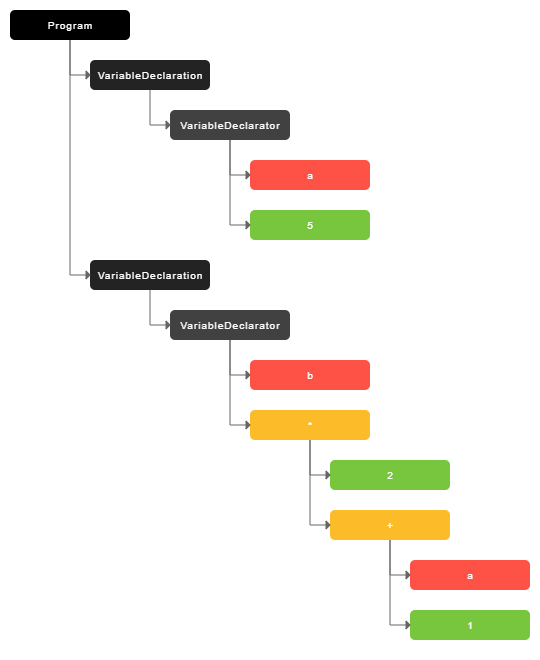
\includegraphics[scale=0.6]{img/ast.png}
  \caption{Пример абстрактного синтаксического дерева}
  \label{ast}
\end{figure}

На рисунке \ref{ast} представлен пример абстрактного синтаксического дерева, построенного для 
следующего фрагмента кода на языка JavaScript:
%  Дерево было построено с использованием парсера,
% входящего в состав транспайлера Babel. 

\lstinputlisting[language=JavaScript, style=linesWithNumbers]{listings/ast-expression.js}

Дерево было построено с использованием парсера, входящего в состав транспайлера Babel.

После того, как было получено представление о понятии AST, можно перейти к обзору основных этапов 
работы Babel, которые представлены на рисунке \ref{babel_stages}.
\begin{figure}[h!]
  \centering
  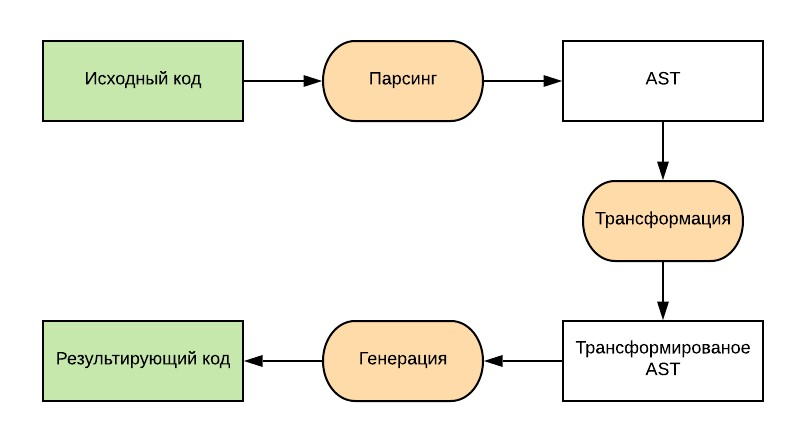
\includegraphics[scale=1.2]{img/babel_stages.jpg}
  \caption{Этапы работы Babel}
  \label{babel_stages}
\end{figure}

\subsubsection*{Парсинг}
На этом этапе код, передаваемый в Babel, конвертируется в абстрактное синтаксическое дерево. 
В свою очередь этап парсинга подразделяется на 
две фазы: \textit{лексический анализ} и \textit{синтаксический анализ}.

В ходе лексического анализа текст исходного кода преобразуется в массив токенов. По этой причине фазу 
лексического анализа часто называют токенизацией. Здесь токен - это объект, описывающий любую значащую 
подпоследовательность символов исходного кода. Например, фрагмент кода

\lstinputlisting[language=JavaScript, style=linesWithNumbers]{listings/fragment-for-tokenization.js}
будет преобразован в следующий массив токенов:

\lstinputlisting[language=JavaScript, style=linesWithNumbers]{listings/tokens.js}
Свойства start и end описывают положение токена в строке, loc $-$ строку, в которой был найден токен. 
Поле type указывает на объект, который хранит набор свойств, описывающих каждый отдельный токен:
\lstinputlisting[language=JavaScript, style=linesWithNumbers]{listings/token-type.js}

Далее следует так называемый синтаксический анализ, цель которого $-$ построение абстрактного 
синтаксического дерева на основе массива токенов, полученного на предыдущем этапе. В ходе этого 
процесса токены преобразуются в узлы дерева (Node), которые кроме уже описанных данных содержат также
информацию о типе узла. Примерами таких типов являются FunctionDeclaration, VariableDeclaration или 
ReturnStatement. Для рассмотренного выше фрагмента кода построенное парсером абстрактное синтаксическое 
дерево будет выглядеть следующим образом:

\lstinputlisting[language=JavaScript, style=linesWithNumbers]{listings/ast-for-fragment.js}

\subsubsection*{Трансформация}
Как только абстрактное синтаксическое дерево построено, начинается этап трансформации. На этом этапе 
производится рекурсивный обход, во время которого добавляются, заменяются или удаляются узлы дерева.
Трансформации, проводимые над деревом, определяются списком подключенных плагинов и применяются в 
порядке их следования в этом списке.

*Используется Посетитель, подробности далее* 

\subsubsection*{Генерация}
По окончании модификации, абстрактное синтаксическое дерево конвертируется обратно в код. 
Происходит это следующим образом: производится обход дерева в глубину, в процессе которого строится строка,
представляющая модифицированный код.

\subsubsection*{Шаблон Посетитель}

Обход абстрактного синтаксического дерева, производимый на этапе трансформации, реализован с применением 
шаблона проектирования Посетитель. Это поведенческий шаблон проектирования, впервые описанный в книге 
``Приёмы объектно-ориентированного проектирования. Паттерны проектирования'' \cite{gang_of_4}.
Суть шаблона заключается в предоставлении возможности определять новые операции над объектами,
 не внося изменения в классы этих объектов.

% \subsubsection*{Решаемая проблема}
Проблема, которую решает шаблон Посетитель, можно сформулировать следующим образом:

Необходимо определить ряд несвязанных между собой операций над объектами, принадлежащими определенной структуре.
При этом, требуется избежать модифицирования кода классов этих объектов при добавлении новых операций. 

Шаблон Посетитель описывает решение этой проблемы так:
вместо того чтобы добавлять новое поведение в каждый объект структуры, необходимо вынести это поведение 
в отдельный класс посетителя. Таким образом объекты не будут выполнять операции самостоятельно, а вместо этого 
они будут передаваться в методы посетителя.

Посетитель, в свою очередь, будет содержать множество методов, обрабатывающих объекты разных типов, так как
поведение для них скорее всего будет отличаться. Вопрос, какой именно метод вызывать для каждого конкретного объекта,
разрешается с помощью механизма двойной диспетчеризации. Ответственность за вызов правильного метода посетителя
возлагается на сам объект, передаваемый посетителю в качестве аргумента. Для этого в каждом классе структуры
определяется специальный метод \code{accept(Visitor v)}, внутри которого происходит вызов метода посетителя, соответствующего
типу данного объекта.

На рисунке \ref{visitor_uml} представлена UML диаграмма, иллюстрирующая классическую реализацию шаблона
Посетитель. Диаграмма состорит из следующих компонентов:
\begin{itemize}
  \item \textbf{Visitor} $-$ описывает общий интерфейс для всех посетителей. Содержит объявления 
    методов \code{visit} для каждого конкретного типа элементов. 
  \item \textbf{ConcreteVisitor} $-$ конкретный класс посетителя, реализует интерфейс, определенный в Visitor.
  \item \textbf{Element} $-$ интерфейс, содержащий объявление метода \code{accept}.
  \item \textbf{ElementA / ElementB} $-$ конкретные классы элементов структуры, реализуют метод \code{accept}
    интерфейса Element, вызывая внутри него метод Посетителя, соответствующий своему типу.
  \item \textbf{Client} $-$ класс-пользователь структуры объектов. В нем происходит вызов метода \code{accept}
    объекта с конкретным экземпляром Посетителя.
\end{itemize}

\begin{figure}[h!]
  \centering
  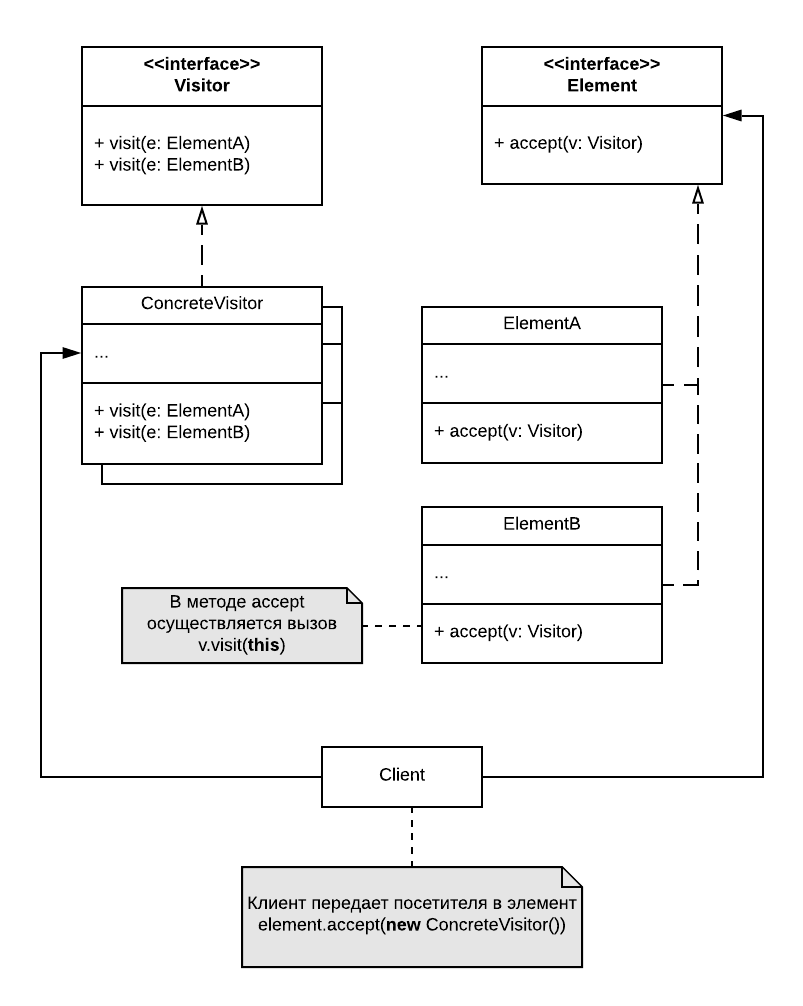
\includegraphics[scale=1.0]{img/visitor_uml.png}
  \caption{UML диаграмма компонентов шаблона Посетитель}
  \label{visitor_uml}
\end{figure}

Шаблон Посетитель широко используется в реализация различных компиляторов для определения операций над 
абстрактными синтаксическими деревьями. Babel, компилирующий JavaScript код в другой JavaScript код,
также не является исключением. Однако, из-за ограничений языка программирования JavaScript, таких как
отсутствие поддержки перегрузки методов и возможности определять интерфейсы, реализация шаблона Посетитель
в Babel несколько отличается от классической.

В Babel посетить представляет из себя обычный JavaScript объект, который содержит методы, чьи названия 
совпадают с типом узлов AST, которые они ``посещяют''.

\lstinputlisting[language=JavaScript, style=linesWithNumbers]{listings/visitor_expample.js}

Внутри методов Посетителя определяются операции, которые необходимо произвести над узлами данного типа.
Узлы абстрактного синтаксического дерева в Babel не содержат метода \code{accept}. Вместо этого за вызов
подходящего метода Посетителя отвечает функция \code{traverse}, выполняющая обход дерева. Ниже приведен 
псевдокод, упрощенно иллюстрирующий механизм работы этой функции.

\lstinputlisting[language=JavaScript, style=linesWithNumbers]{listings/traverse.js}
 *Плагины Babel - это по сути визиторы*
\pagebreak

\begin{thebibliography}{9}
  \bibitem{ecma-262} Стандарт ECMA-262 [Электронный ресурс] $-$ Режим доступа: \linebreak
    \url{https://www.ecma-international.org/publications/standards/Ecma-262.htm}
  \bibitem{documentation} Документация Babel [Электронный ресурс] $-$ Режим доступа: \linebreak
    \url{https://babeljs.io/docs/en}
  \bibitem{traceur} Документация Traceur [Электронный ресурс] $-$ Режим доступа: \linebreak
    \url{https://github.com/google/traceur-compiler/wiki/Getting-Started}
  \bibitem{jstransform} Репозиторий JSTransform на сервисе GitHub [Электронный ресурс] $-$ Режим доступа:
    \url{https://github.com/facebookarchive/jstransform}
  \bibitem{gang_of_4} Э. Гамма, Р. Хелм, Р. Джонсон, Д. Влиссидес. Приёмы объектно-ориентированного проектирования. Паттерны проектирования, СПб.: Питер, 2017. $-$ 368 с.: ил.
\end{thebibliography}
\end{document}